\documentclass[12pt,a4paper]{article}
\usepackage[utf8]{inputenc}
\usepackage[toc,page]{appendix}
\usepackage{amsmath}
\usepackage{amsthm}
\usepackage{amsfonts}
\usepackage{amssymb}
\usepackage[overload]{empheq}
\usepackage{color}
\usepackage[dvipsnames]{xcolor}
\usepackage{fullpage}

\title{branch and bound pour 01UKP}
\author{Dorian Dumez}

\begin{document}
\maketitle

\section{Le code}
Ces algorithmes ont été implémentés en Julia, basé sur ceux que vous nous aviez fournis.

\subsection{Le travail du TP}
La première partie du main correspond à un travail que vous nous aviez demandé en TP. Les données du problème sont donc rentré en dur dans une instance. Ensuite une solution est construite par un algorithme glouton avant d’être amélioré de manière heuristique. Ces résultats étant mis en regard avec une borne duale (la relaxation linéaire) pour cette instance.\\

\subsection{La fonction de branch and bound}
La fonction de branch and bound est contenu dans les fichier "branchandbound.jl".\\

Cette fonction prend en paramètre l'instance du problème, la solution courante sur laquelle on travaille (une solution ne contenant aucun objet est passé en paramètre lors de l'appel de la fonction dans le main). On a aussi un entier k correspondant à l'indice de l'objet (dans la solution et l'instance) que l'on est en train de considérer. Enfin on garde en mémoire la meilleure solution trouve actuellement (une solution ne contenant aucun objet est passé en paramètre lors de l'appel de la fonction dans le main). De plus pour éviter de ré-écrire la fonction pour toutes les bornes, la fonction prend en paramètre la fonction qui va calculer la borne duale (cette dernière prend en paramètre l'instance, la solution courante et k)\\

Cette fonction est récursive et commence par son cas d’arrêt : dans la solution courante tous les objets ont été considérés. C'est le cas si et seulement si l'indice k passé en paramètre (donc l'indice de l'objet que l'on devrai considérer) est supérieur au nombre d'objets. Dans ce cas on compare la solution courante à la meilleure solution dont on dispose (la valeur de la fonction économique étant comprise dans les solutions cette comparaison s’effectue en temps constant), et on retourne la meilleure des deux.\\

Si la solution n'est pas complète, donc que $k \leqslant ukp.n$, on essaye d'ajouter l'objet k. Les objets étant trié par utilité cela correspond au choix glouton. Mais avant d’effectuer l'appel récursif avec ce choix on teste si la borne duale du problème sur cette instance n'est pas inférieure à la valeurs de notre meilleure solution. Ensuite, que l'on ai pu ajouté ou non l'objet, on effectue l'appel récursif sur la solution ne comprenant pas l'objet, toujours sous la condition que sa borne duale ne soit pas inférieure à la valeurs de la meilleure solution. Étant donné que branchandbound renvoi toujours la meilleure solution dont on dispose (durant son cas de base) on peut toujours dire que la meilleure solution dont on dispose est égal à ce que renvoi la fonction. En remarquant que les deux appels récursif sont effectué séquentiellement on vérifie récursivement que la fonction renvoi toujours la meilleure solution don on dispose.\\

\subsection{Les autres fonctions}
On rappelle que les bornes que l'on calcule ne sont valides que si les objets sont triés par utilité.\\

La fonction "trier" contenu dans le fichier "main.jl" sert à ordonner les objets d'une instances par utilité. Elle n'est utilisé qu'une fois par instance, avant tout autre chose après son remplissage. Étant donné son utilisation, sa complexité importe peut donc ce n'est qu'un tri bulle.\\

Toutes les fonctions calculant les bornes duales, et les fonction qu'elles utilisent, sont dans le fichier "relaxation.jl".

La fonction "completeLinear" implémente la borne b1, la borne de Dantzig. Elle va calculer l’objet critique s compte tenu des objets déjà assigné dans la solution. C'est à dire qu'elle va chercher l'objet s du sous-problème avec $ukp.n - k$ variables (les k premières variables étant déjà assignés on ne les considères pas) et de capacité $ukp.W - taille(solution courante)$. Une fois l'indice s de l'objet critique calculé on peut directement calculer la valeur de notre borne duale (en prenant bien garde au cas où un tel objet n'existe pas, c'est a dire si la contrainte de capacité du sous-problème n'est pas restrictive).\\

La fonction "completeMetT" implémente la borne b2, celle proposé par Martello et Toth en 1977. De la même manière que "completeLinear", cette fonction va commencer par calculer l'objet critique s par rapport à la solution courante. Puis, si ces objets existent, calculer les incréments $U^0$ et $U^1$ (sinon on les fixes à 0). Avant d'ajouter le plus grand d'entre eux à la solution courante à laquelle on a greffé un choix glouton.\\

La fonction "completeMetT2" implémente la borne b3, la borne de Martello et Toth amélioré proposé dans le chapitre 2 de leur livre "knapsack problem". Comme précédemment on calcule l'objet critique s. Ensuite on calcule les objets $\sigma^2(s)$ et $\sigma^1(s)$ à l'aide des fonction du même nom. Mais ces bornes ne peuvent être calculé en considérant les objets déjà fixé par la solution courante car il la modifie. Pour finir les deux incréments $U^0$ et $U^1$ sont calculés si les objets qu'ils nécessite existent et la fin est la même manière que pour la fonction "completeMetT".\\

\section{Expérimentations}
Toutes les expérimentations sont faites dans le fichier "main.jl". \\

\subsection{Le travail du TP}

L'instance de cours est en dur dans le code. Une solution gloutonne est calculé pour cette instance est calculé avant d’être amélioré de manière heuristique et mis en regard avec la borne duale de la relaxation linéaire et de la solution exacte calculé par branch and bound.\\

Cette exemple nous laisse à penser que la construction et l'amélioration heuristique est une bonne piste car il amène à une solution d'une valeur de 105 alors que la solution exacte est a 107, soit une différence de $1,87 \%$. De plus la borne duale semble aussi être de bonne qualité car elle correspond à la solution optimale, modulo l’arrondit à l'entier inférieur.\\

\subsection{Vérification des algorithmes}

Pour vérifier que les 3 algorithmes de branch and bound donnent une solution optimale un jeux de 8 instances de tests représentatif, fournit avec une solution optimale, est utilisé. La solution optimale des 3 versions du branch and bound est comparé à cette solution optimale fournie.\\

\subsection{Montée en charge}
Toutes les instances utilisé pour la montée en charge sont celle que vous nous avez fournit.\\

La troisième variante du branch and bound a été exclue des tests de performances car elle c'est révélé clairement en deçà de ses concurrents. Cela s'explique par coût de calcul important de la borne 3, à mettre en regard avec l'agressivité avec laquelle on l'utilise. De plus elle s'adapte beaucoup moins à la solution courante que ces deux prédécesseurs. En effet les deux bornes précédentes semble être de bonne qualité donc celle ci ne peut pas beaucoup les améliorer et ne le fait sans doute même pas à cause de son manque d'adaptabilité.\\

Les moyennes des tests suivant sont toujours effectué sur 5 instances différentes du même type. Les jeux d'instances présente différents paramètre tels que le nombre de variable, le domaine de leur poids et coût et les différentes corrélations possible.\\

~\\
\begin{figure}[h]
	\centering
	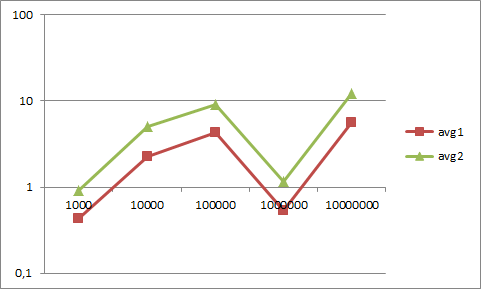
\includegraphics{./resultat/graphe_temps_selon_coef_range_(correlation_type_3_200_variables).png}
	\label{fonctrange}
	\caption{temps d’exécution en fonction de la taille des domaines}
\end{figure}
~\\

Donc de manière générale la taille du domaine semble complexifier la résolution des instances. Ces moyennes sont en secondes sur des instances avec un corrélation de type 3 et 200 variables.\\

~\\
\begin{figure}[h]
	\centering
	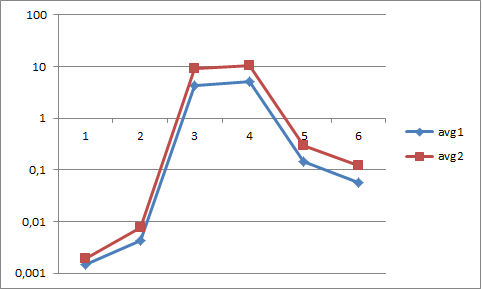
\includegraphics{./resultat/graphe_temps_selon_corelation_(coef_range_100000).png}
	\label{fonctcore}
	\caption{temps d’exécution en fonction du type de corrélation}
\end{figure}
~\\
\begin{figure}[h]
	\centering
	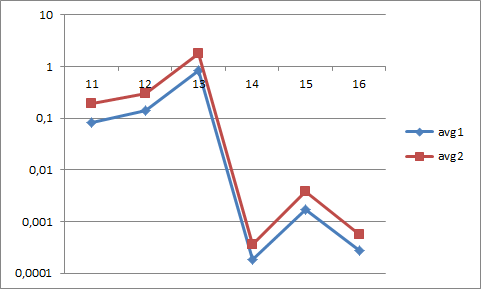
\includegraphics{./resultat/analyse_instances_hard_temps_selon_type(50_variables).png}
	\label{hard}
	\caption{temps d’exécution en fonction du type de corrélation sur des instances difficiles}
\end{figure}
~\\
~\\

Ceci nous permet de conclure que la corrélation entre les différents coefficient joue un rôle très important sur les temps de résolution. Les tests de la courbe \ref{fonctcore} on été effectué sur des instances à 200 variables avec des domaines de taille 100 000. Ceux de la courbe \ref{hard} avec des instances à 50 variables sur des domaines à 1 000 éléments.\\

\section{Conclusion}

Dans tout les cas la première variante semble être la plus performante. En effet la borne utilisé est déjà de bonne qualité et est très rapide à calculer. La deuxième bien que légèrement meilleure est aussi plus longue à calculer donc cela se ressent sur les temps d’exécutions.\\

Attention : toutes les instances non utilisées par les réglages actuels des tests de performances ont été supprimés pour respecter la contrainte de taille du rendu imposé par madoc.

\end{document}